% !Mode:: "TeX:UTF-8"
% !TEX root = ..\Literature_Translation.tex
%% 文献翻译中使用的标题
\newcommand\kchapter[1]{\stepcounter{chapter}\chapter*{\the\value{chapter}#1}}
\newcommand\ksection[1]{\stepcounter{section}\section*{\xiaosi\the\value{chapter}.\the\value{section}#1}}
\newcommand\ksubsection[1]{\stepcounter{subsection}\subsection*{\wuhao\the\value{chapter}.\the\value{section}.\the\value{subsection}#1}}

%%文献翻译中需要的计数器
\captionsetup{figurewithin=none,tablewithin=none}
\newcounter{app}
\renewcommand{\theapp}{\Alph{app}}
\renewcommand{\thefigure}{\theapp-\arabic{figure}}
\renewcommand{\thetable}{\theapp-\arabic{table}}
\renewcommand{\theequation}{\theapp.\thechapter.\arabic{equation}}

%% 文献翻译环境
\newenvironment{transcript}{
%  \setcounter{tocdepth}{-1} 
  \onequarterspacing
  \begingroup
  \let\clearpage\relax %
  \CTEXsetup[name={,},number=\arabic{chapter},format={\zihao{4}\heiti\bfseries},nameformat={\zihao{4}\heiti\bfseries},titleformat={\zihao{4}\heiti\bfseries},numberformat={\zihao{4}\heiti\bfseries},beforeskip=10pt,afterskip=10pt]{chapter}
  \CTEXsetup[format={\zihao{-4}\heiti},nameformat={\zihao{-4}\heiti},titleformat={\zihao{-4}\heiti},numberformat={\zihao{-4}\heiti},beforeskip=0pt,afterskip=5pt]{section}
  %\titleclass{\chapter}{straight}  %%不换页!!
  %\titleformat{\chapter}[block]{\singlespacing\sihao\heiti\bfseries}{\thechapter}{1ex}{}{}
  %\titlespacing{\chapter}{0pt}{2em}{1em}
  %\titleformat{\section}[hang]{\singlespacing\xiaosi\heiti}{\thesection}{1em}{}{}
  %\titlespacing{\section}{0pt}{0.8em}{0.1em}
  %\titleformat{\subsection}[hang]{\singlespacing\wuhao\heiti}{\thesubsection}{1em}{}{}
  %\titlespacing{\subsection}{0pt}{0.5em}{0.5em}
}{\endgroup}
\newpage
\begin{transcript}
	\kappendix[chapter]{文献翻译}

	% !Mode:: "TeX:UTF-8"
% !TEX root = ..\Literature_Translation.tex
\stepcounter{app}
\begin{Abstract}
\chapter*{某装配车间批调度案例研究}\addcontentsline{toc}{section}{某装配车间批调度案例研究}
\begin{center}
\vspace{2mm}
{
 {\xiaosi Rock Lin, Ching-Jong Liao}

 {\xiaowu Department of Industrial Management, National Taiwan University of Science and Technology, Taipei 106, Taiwan}
}
\end{center}
{\songti
\noindent \xiaowu\textbf{摘要:}本文探讨了在某机械工厂装配车间内的生产调度问题。该装配工艺包含两个工段:在工段1,所需零件在一批同速机上同时装配,并且这些同速机的准备时间也相同;装配完成的部件进入工段2 进,并在不同的异速机上进行系统集成组装。同速机和异速机在切换生产产品簇的时候都需要考虑换线时间。本文建立了一个混合整数规划(MIP) 模型以求解小型问题,并提出了用于求解中、大型问题的三个启发式方法。经过计算检验,相比较其余两个方法,其中一个利用滚动时域调度策略的整批产品簇排序启发式组合的方法(RFBFS),在解决问题方面有较高质量。实践表明,RFBFS方法确实显著优于现行方法。

\keywords{混合整数规划、作业划分、批量作业、产品簇调度}
}
\end{Abstract}

\kchapter{引言}
在机械制造工厂中,经常会遇到批调度问题,我们将在本文具体研究工厂中的两阶段组装车间的调度。这个问题与Yokoyama 等的论文中所描述的两阶段组装车间调度问题类似:工段1,生料组装成产品部件;工段1,这些部件装配成产品。然而,由于技术与工艺十分复杂,生料的组装不仅困难,而且成本高,这便是通常情况下,企业将生料组装外包(或直接采购组装件)的原因。因此,我们为这个装配车间构建成一个两阶段流水车间模型,在工段1 进行模块化装配,在工段1 进行系统集成。

随着20年的技术不断革新,需求的多样性也水涨船高,产品便不断向着多功能、高性能的要求发展,这使得机械化生产变得日益复杂。如此背景下,工厂的车间管理不得不处理好下列调度问题:
\begin{compactenum}[(1)]
\item 如何缩短生产周期?
\item 如何减少在制品(WIP)?
\item 如何实现及时交货?
\item 如何处理紧急插单?
\end{compactenum}

本文的研究对象为台湾的一家机械厂——峰明机械有限公司,该工厂能按订单制造10 余种塑料袋生产机。目前,这些订单是按照最早交货期(EDD)规则安排生产的。为了快速响应客户需求,一件产品(一项作业)将由多位操作者在一个作业场所内同时组装(如\reff{fig:cwf}所示)。
由于空间限制,操作者之间产生干涉,并因此产生了闲置和等待时间。为了减少闲置和等待时间,我们提出了作业划分策略(源于多批次发货概念)和批量作业以提高车间生产效率。为缩短制造期,我们同时也运用了产品簇调度的方法:同簇产品作业群组成一批,以消除产品簇换线时间。如\reff{fig:bwf} 所示,工段1 设置成批量处理机器,c 位熟练工可以同时分开组装c个工件。工段2设置成离散机器,工件进入机器后按工序处理,然后一个接一个离开机器。
\begin{figure}[h]
\begin{floatrow}[2]
\centering
\ffigbox{\caption{当前制造流程}\label{fig:cwf}}{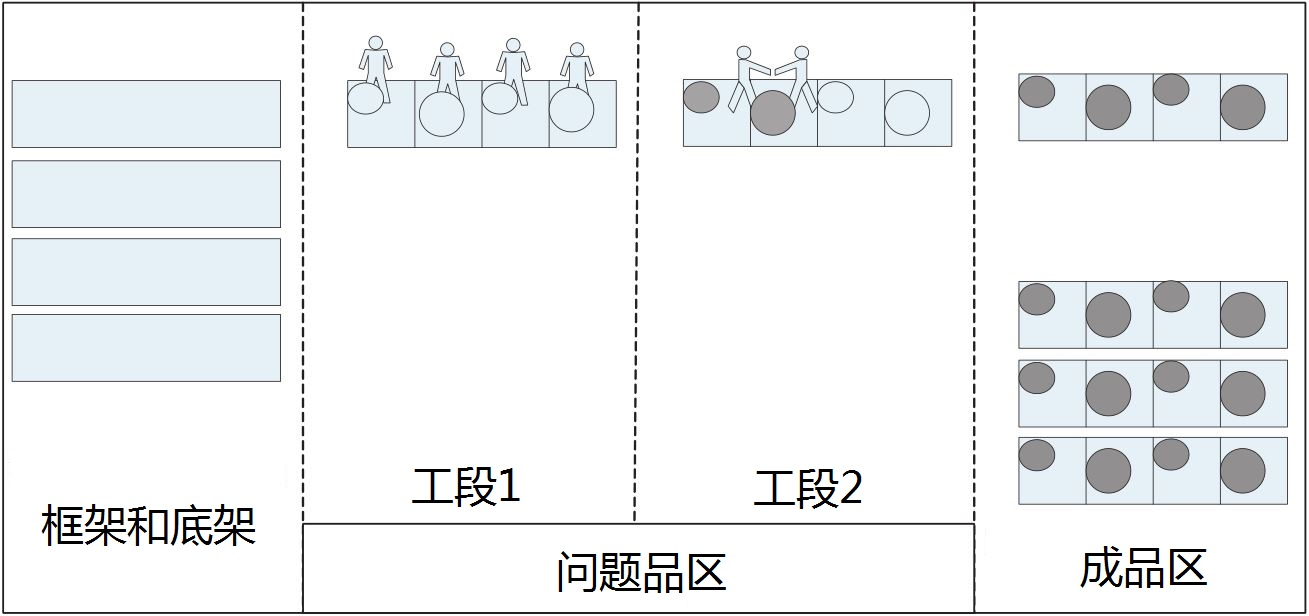
\includegraphics[width=8cm]{current_work_flow.jpg}}
\ffigbox{\caption{运用了作业划分和批量作业的制造流程}\label{fig:bwf}}{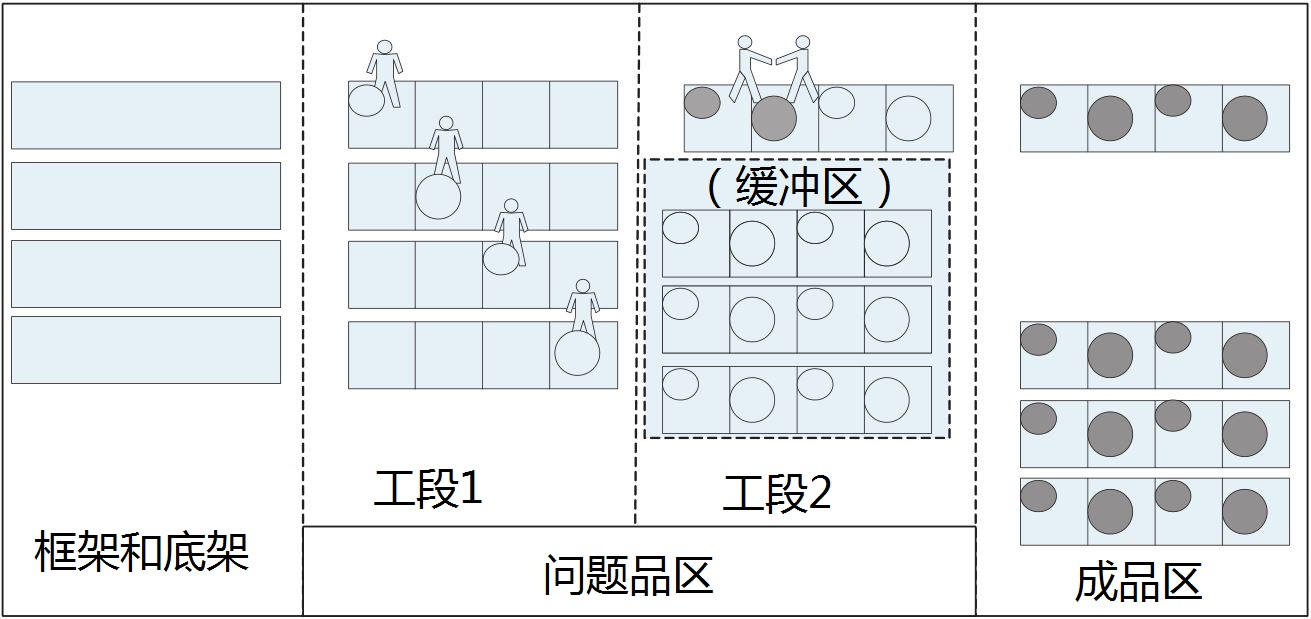
\includegraphics[width=8cm]{batch_work_flow.jpg}}
\end{floatrow}
\end{figure}
如此一来,可以减少大量由于工段1 中互相干涉产生的闲置时间,同时,产品簇调度可以减少两个工段的作业换线时间和产品簇换线时间。

通常可以建立目标函数来评估调度方案方法的运行效果。本文中假设同一批次工序作业换线时间相同,同一产品簇的簇换线时间相同。不过这样的作业划分可能会耽搁其他作业进程,甚至使其延迟交货。为了权衡,我们将引入多个目标,包括制造期、总完工时间和同延迟时间,这些目标间包含相左的方法以评估所提解决方法的性能。

所考虑的问题的主要特点是批量作业。Potts 和Kovalyov(2000)在其文中所回顾的批调度问题反映了大量文献研究,这些研究使得批量决策的调度模型变得完整。Lee(1992),Webster 和Baker(1995),Potts(2001)以及Neale 和Duenyas(2000) 将预烧炉构建成批量处理机器模型,并改良了方法,使之在评估生产周期和(或)流程时间取得较好效果。
一个批量作业机器可以同时加工处理多项作业,并且加工时间为所有作业中最长的加工时间。
Ahmadi(1992)首次考虑了具有批量和离散机器的加工系统,系统中每一个批量处理机器至多可同时处理c项作业。他们提出了全批量最短加工时间(Full Batch-SPT) 和全批量交易(Full Batch-Dealing)规则以求解最小完工时间和问题。他们也提出了Johnson 最长加工时间(LPT-Johnson)法则以求解多产品簇作业系统的最小制造期问题。
Hoogeveen 和 van de Velde(1998)拓宽了Ahmadi 的成果,利用定位完成时间的概念呈现了有效的拉格朗日下界。Kim(2002)还解决了批量理算系统的调度问题,以最小化完工时间和。Gong(2010)考虑了两阶段流水车间问题,机器1受到阻塞约束,机器2是具有相同换线时间的离散机器。他们证实,当目标是制造期最小化时,这是一个NP-hard 问题。Liu(2009) 研究了加工时间相同的单批量处理机器的作业调度问题,他们建立了一些适用于包括最小加权完成时间和、最大延迟以及滞后和问题的有效算法。
此外,Schaller(2007)发现若考虑换线时间,在单机器情况下,最小滞后和是NP-hard 问题,因为仅单机器情况下的最小滞后时间和已经是NP 困难了,这以及被Du 和Leung(1990) 所证明。

总的来说,被考虑的调度问题建立成为一个两机器流水车间系统模型,集成了一个具有相同批量换线时间常量的批量处理同速机,这些机器的后续为离散异速机。这两种机器在处理作业切换时都需考虑产品簇换线时间。
调度的目标是最小化加权制造期和、完工时间和以及滞后时间和。但这是个NP-hard 问题,因为不考虑换线的最小完工时间和的特例下,已被Ahmadi(1992)证明是NP-hard 了。这个问题的NP 困难也可被看作基于这个特例事实:Du 和Lenug(1990) 证明了最小化滞后时间和的单机是NP-hard 问题。

余下全文如是安排:我们将在第2节通过一个工厂案例描述现行调度方法;在第3节,批调度模型中将集成作业划分概念,并将对此提供一个混合整数规划(MIP) 模型,同时,我们也将建立3个针对中、大型问题的启发式方法;第4节将通过数值计算实验和实践运用来评估这些启发式发发的效果;最后,我们将在第5节总结。

% !Mode:: "TeX:UTF-8"
% !TEX root = ..\Literature_Translation.tex
\kchapter{现行调度方法}
下面将引入相关符号,并对案例中的工厂所运用的现行调度方法进行描述。
\ksection{符合说明与相关假设}
为了方便问题描述,符号说明如下:\\[5pt]
%\begin{center}
\begin{supertabular}{ll}
$j$ & 作业标记 \\
$i$ & 批次标记\\
$r$ & 批次中的位置标记\\
$b$ & 工段中的批数,$b\geqslant2$\\
$c$ & 工段1的批量\\
$J$ & 需要调度的作业集合,$J=\{1,2,...,n\}$\\
$p_{aj}$ & $J_j$在工段$1?a$的单件处理时间,$p_{aj}=p_a$\\
$p_{1j}$ & $J_j$在工段1的处理时间,$p_{1j}=p_1$\\
$p_{2j}$ & $J_j$在工段1的处理时间\\
$s_a$ & 在工段1的作业换线时间\\
$s_b$ & 在工段2的批次换线时间\\
$s_{f1}$ & 在工段1的产品簇换线时间\\
$s_{f2}$ & 在工段2的产品簇换线时间\\
$f_j$ & $J_j$的产品簇,$f_j=1,2,3,4$\\
$f_{1,[i,r]}$ & 在工段1中安排在第$r$批次作业$[i,r]$的产品簇 \\
$f_{2,[j]}$ & 在工段2中安排在第$j$批次$J_{[j]}$的产品簇 \\
$k_{1,[i,r]}$ & \begin{numcases}{=}
{\liuhao 0 }&{\liuhao 在工段1,如果作业$[i,r]$和它的前继作业同属一个产品簇}\notag\\
{\liuhao 1 }&{\liuhao 其他情况} \notag
\end{numcases}\\[5pt]
$k_{2,[j]}$ & \begin{numcases}{=}
{\liuhao 0 }&{\liuhao 在工段2,如果$J_[j]$和它的前继作业同属一个产品簇}\notag\\
{\liuhao 1 }&{\liuhao 其他情况} \notag
\end{numcases}\\
$S$ & 已调度的作业集合\\
$S_U$ & 未调度作业集合\\
$B$ & 已调度批集合\\
$B_i$ & 工段1的第$i$批,$B_i\subset B$\\
$p_1(B_i)$ & 工段1的$B_i$处理时间\\
$D_j$ & $J_j$的交货期\\
$d_j$ & $J_j$的工期\\
$d_{[j]}$ & $J_{[j]}$在工段2的工期\\
$C_{1,[i]}$ & 批$i$在工段1的完工时间\\
$C_{2,[j]}$ & $J_{[j]}$在工段2的完工时间\\
$T_j$ & $J_{[j]}$的滞后时间\\[10pt]
%$$ & \\
\end{supertabular}
%\end{center}

下面是该问题的相关假设:
\begin{itemize}
\itemsep=0pt\parskip=0pt
\item 所有作业在0时刻皆未被占用;
\item 作业总量可被批量大小$c$整除,即$n=b\times c$;
\item 批次中的作业需在工段1处理完该批后方可开始工段2的处理;
\item 工段1中处理单件需要考虑作业换线时间$s_a$;
\item 工段1上的批量处理需要考虑批量换线时间$s_b$;
\item 新产品簇在工段1上加工前需要考虑产品簇换线时间$s_{f1}$;
\item 新产品簇在工段2上加工前需要考虑产品簇换线时间$s_{f2}$;
\item 事先已获得固定的处理时间、换线时间和交付期。
\end{itemize}
\ksection{生产制造过程}
为了简化流程和扩大生产能力,所有零件、组装子件全部外包给资深的合作伙伴或零售商。因此,该生产系统可以被构建成一个两阶段装配流水车间:
\begin{inparaenum}[(1)]
\item 一个组装工段,用来将零部件、模块等组装成框架;
\item 一个集成工段,应用了机械电子工程(M\&E)的集成手段。
\end{inparaenum}
应用模块化设计和标准化以允许所有产品共享同条生产线,并且有着相同的生产时间。如此一来,所有产品都可由11个子系统构成,如\reft{tab:11+4}所示。
\begin{table}[h]
  \centering\xiaowu
  \caption{11个子系统和4个作业块(A,B,C,D)}
    \begin{tabular}{llllll}
    \toprule
    \multicolumn{2}{c}{前部} & \multicolumn{2}{c}{中部} & \multicolumn{2}{c}{后部} \\
    \midrule
    A-1   & 推辊机   & B-1   & 水平电子码(EPC)机 & D-1   & 袋酱机 \\
    A-2   & 张力锟机  & B-2   & 垂直电子码(EPC)机 & D-2   & 冲孔机 \\
    A-3   & 压袋机   & B-3   & 封刀机   & D-3   & 输送机 \\
    A-4   & 送料机   & C-1   & 摇摆系统  &       &  \\
    \bottomrule
    \end{tabular}%
  \label{tab:11+4}%
\end{table}%
需要考虑各子系统的负荷和操作进程,以平衡产线和缩短完工时间(Nearchou,2011)。所有的操作被分解成4个操作块(A,B,C,D),并且分别指派给4位一组中的熟练工。这4位工人将框架和底架移至工段1的同一个区域以开始作业的操作,同时他们需要准备好操作的所需部件和工具。而后,他们便开始在各自的操作块中进行组装。
由于空间限制,组装操作很容易产生人员间的干涉,并会由此产生潜在的等待时间,这常常会导致生产瓶颈。
每当作业在工段1的组装操作结束,便会转移到工段2,由2位该组的熟练工继续作业。他们运用机电集成技术,包括伺服或计算机系统安装、参数设置、调试等。之后,完成的作业被移至成品区。

\ksection{换线时间和产品簇}
大多数有关调度的研究将换线时间看做是可忽略或者将其算作处理时间的一部分(Logendran,2005;Allahverdi,1999),但是在此案例中,换线时间是很重要的,不得不考虑。此处,换线时间可以归为两类:
\begin{inparaenum}
\item 作业换线,作为工作准备,将所有要处理作业的零部件置好;
\item 产品簇换线,用于获得工具、调整工装夹具、检查不同产品簇的需要加工零部件(Eren,2007)。
\end{inparaenum}
工段1在操作开始前,需要一个作业换线时间$s_a$,而当开始第1个作业或切换产品簇的时候,在两个工段都需要考虑产品簇换线时间$s_{j1}$和$s_{j2}$。简化起见,我们假设这些都是常数,即$s_a=5.2\ h$,$s_{f1}=3.2\ h$,$s_{f2}=1.6\ h$。如\reft{tab:2yearproduction}所示,现有超过10个模块在案例工厂加工,并且这些作业可以根据模块属性群组为4个产品簇($f_1\sim f_4$)。需要注意作业处理时间不包括换线时间$s_a$,因为它需要和批次换线时间换线时间$s_b$作比较。
\begin{table}[htbp]
  \centering\xiaowu
  \caption{近两年作业的模块和产品簇的产量}
    \begin{tabular}{lrcccc}
    \toprule
    \multicolumn{2}{c}{模块} & \multicolumn{2}{c}{数量} & \multicolumn{2}{c}{处理时间(h)} \\
    \midrule
    \multicolumn{1}{l}{编号} & \multicolumn{1}{c}{产品簇 } & 2007  & 2008  & $p_1/1$位工人 & $p_2/2$位工人 \\
    \midrule
    900BR & \multicolumn{1}{c}{$f_1$} & 26    & 15    & 24    & 16 \\
    1000DT & \multicolumn{1}{c}{$f_1$} & 30    & 46    & 24    & 16 \\
    800ST2 & \multicolumn{1}{c}{$f_2$} & 44    & 51    & 24    & 12 \\
    1100ST3 & \multicolumn{1}{c}{$f_2$} & 18    & 11    & 24    & 12 \\
    1000TT & \multicolumn{1}{c}{$f_3$} & 43    & 30    & 24    & 8 \\
    800TT & \multicolumn{1}{c}{$f_3$} & 37    & 31    & 24    & 8 \\
    1000VV & \multicolumn{1}{c}{$f_4$} & 21    & 47    & 24    & 10 \\
    其他 & \multicolumn{1}{c}{$f_4$} & 49    & 67    & 24    & 10 \\
    \multicolumn{2}{c}{平均值(每月)} & 22.33 & 24.83 & -     & - \\
    \bottomrule
    \end{tabular}%
  \label{tab:2yearproduction}%
\end{table}%

\ksection{目标函数}
如引言所述,用制造期、完工时间和、滞后时间和等多目标加权求和可以更好地展现该问题,即:
\[Z=\alpha C_{\max}+\beta\sum_{j=1}^n C_{2,[j]}+\gamma\sum_{j=1}^n T_j
\]
式中的$\alpha,\beta,\gamma$位非负权重系数,可以用下面的法则确定:
\begin{compactenum}[(1)]
\item $C_{\max}$和$\sum C_{2,[j]}$不一定有相同的值域。为了减小差异,可以采用Framinan(2002)提出的调节程序。先假设一项有n个独立作业工作的期望完成时间为$C_{\max}/2$,因此$nC_{\max}\approx\sum C_{2,[j]}$,相当于将$C_{\max}$和$\sum C_{2,[j]}$与$n/2$和$1$分别相乘。
\item 实践中,权重系数的确定很大程度上取决于决策者(Taboada 和Coit,2008)。在案例的工厂中,完工时间和可以帮助评估及时交付情况,而滞后时间和主要作为超时加班计划的目的。一版安排完工时间和与滞后时间和为制造期的2倍。所以,$C_{\max},\sum C_{2,[j]}$和$\sum T_j$需分别再乘以1,2,2。如$n=12$,则权重为$(\alpha,\beta,\gamma)=(6,2,2)=(0.6,0.2,0.2)$。
\end{compactenum}
\ksection{现行调度方法}
现行的调度方法工作流程如\reff{fig:csf}所示。
\begin{figure}[h]
\centering
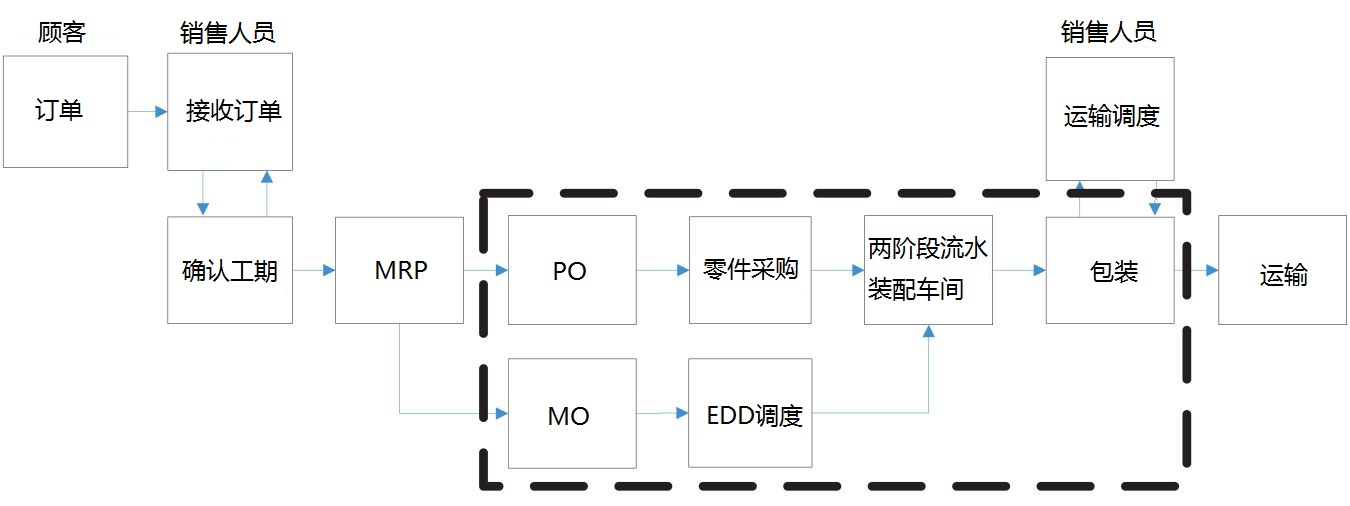
\includegraphics[width=16cm]{current_flow.jpg}
\caption{现行调度方法工作流程\label{fig:csf}}
\end{figure}
生产管理员确认了交付期后,销售人员接受顾客的订单并将订单通知发给生产管理员。当订单通知下达车间时,MRP 中心发布采购订单(PO)和制造单(MO)。通常工期以周计算,要比交付期$(D_j)$提前$5\ days\times 8\ h=40\ h$,即$d_j=D_j-40$。所有的采购订单需以PO 的基础立即呈给供应商,同时,生产调度需立即按MO 的基础制定。目前,作业的顺序按EDD 分派规则制定,并且单件流(Li 和Rong,2009)将在两个工段按相同顺序执行。

当换线时间等于0时,EDD 规则是最小化最大延迟的最优解(Baker 和Magazine,2000)。然而,现今的车间中,许多作业换线时间和产品簇换线时间会在单件流的情况下产生,所以EDD 规则通常会得到较大的完工时间。进一步说,在单件流情况下,4为工人同时在有限的空间内操作(见\reff{fig:cwf}),时常会相互干涉,产生可相当可观的闲置时间,使得处理时间从$p_a=24\ h/4=6\ h$变为$p_a=9\ h$(见\reft{tab:2yearproduction})。因此,现行调度方法将产生下列问题:
\begin{compactenum}[(1)]
\item 单件流会导致物料短缺,产生不能满足调度的处理困难;
\item 频繁换线和闲置使得流程时间变长和更多的超时加班;
\item 由于按期完成率低,不能处理紧急订单。
\end{compactenum}

为了解决这些问题,我们提出了作业划分和批量作业的的策略,将在接下来的章节里讨论。

% !Mode:: "TeX:UTF-8"
% !TEX root = ..\Literature_Translation.tex
\kchapter{建立解决方法}
本章我们将建立该问题的解决方法。首先,我们先将引入作业划分概念,并结合批量作业以减少换线时间、提高装配车间效率。而后,我们建立两个最优化特点,并提出了一个整数规划(MIP)公式以导出最优解。最后,我们提出了三个启发式方法以得到近似最优解。
\ksection{作业划分和批量作业}
为了改善现行的调度方法,我们引入了多批次发货(Bukchin,2002)概念,并打算用作业划分策略将作业划分成几个子作业。将作业划分策略结合入批量处理后,$c$项子作业便可分开同时由$c$个工人来处理。这样一来,可以避免相互干涉,减少等待时间。由于这些子作业都在批量中心,并且是连续离开机器,这$c$位工人必须同时停止作业,否则一些工人可能会处于闲置状态,而另一些工人却还在忙。
可以运用模块化设计和标准化以确保这$c$位工人同时停止作业,这样一来所工作拥有同样的处理时间,$c$位工人可以的工作强度近似一致。
如有必要,这4位工人可以互相帮工,这样一来,这些子作业可以同时完成。
因此,处理可以变得更为流畅,并且在工段1不会产生瓶颈。如\reff{fig:bwf}所示,接下来整个系统可以看作一个两阶段流水车间,工段1有4工人操作的批处理机器,工段2有2工人操作的离散机器。

承前所述,我们在工段1将作业划分成$c$项子作业,必须由$c$位工人同时操作,这样他们可以看作一个容量为$c$项作业的批量处理机器(Liu 和Yu,2000)。批$i$的处理时间为在此批中的最长作业处理时间,即$p_1(B_i)=\max p_{1j}=p_1$。
此外,每当一个新的批量产生,都需要考虑批量换线时间$s_b$,同样,开始首项作业或切换不同产品簇的作业时,需要考虑产品簇换线时间$s_{f1}$。
需要注意的是,批量中的最后一个作业或者同产品簇的下批首个作业不需要考虑产品簇换线时间。如此一来,批次$i$的完工时间$C_{1,[i]}$等于批量启动时间加上批量换线时间加上同批的产品簇换线和作业处理时间,即:
\begin{gather}
C_{1,[0]}=0 \label{equ:1} \\
C_{1,[i]}=C_{1,[i-1]} + s_b + s_{f1}\sum_{r=1}^c k_{1,[i,r]} + p_1 \label{equ:2}\\
(i=1,...,b, \text{如果}f_{1,[i,r]}=f_{1,[i,r-1]}\ k_{1,[i,r]}=0, \text{否则}k_{1,[i,r]}=1 )\notag
\end{gather}

作业在工段2用离散机器处理,作业按批进入但是一个接一个离开。开始首项工作或者切换产品簇的时候需要考虑产品簇换线时间$s_{j2}$。$J_{[j]}$的完工时间$C_{2,[j-1]}$等于$C_{1,[i]}$或者$C_{2,[j-1]}$加上$J_{[j]}$的产品簇换线时间和作业处理时间,即:
\begin{gather}
C_{2,[0]}=0\label{equ:3}\\
C_{2,[j]}=\max\{C_{1,[i]},C_{2,[j-1]}\} + s_{f2}\times k_{2,[j]} + p_{2,[j]}\label{equ:4}\\
(i=1,...,b,j=1,...,n \text{如果}f_{2,[j]}=f_{2,[j-1]}\ k_{2,[j]}=0, \text{否则}k_{2,[j]}=1)\notag 
\shortintertext{如此一来,}
C_{\max}=C_{2,[n]}\label{equ:5}\\
\sum_{j=1}^n T_j = \sum_{j=1}^n \max\{C_{2,[j]}-d_{[j]},0\}\label{equ:6}\\
Z = \alpha C_{\max} + \beta\sum_{j=1}^n C_{2,[j]} + \gamma\sum_{j=1}^n T_j  \label{equ:7}
\end{gather}

为了提高一次完成率,我们只接受滞后和小于$20\ h$每周的调度,因为滞后作业可以适当的周末里加班解决。否则,生产管理员需要和销售人员协商更改滞后作业的完工时间并重新调度。
\ksection{性质发掘}
\newcounter{prop}\newcounter{exam}
%\renewcommand{\theprop}{\arabic{prop}.}
\theoremheaderfont{\heiti}
\newtheorem{propetry}[prop]{性质}
\newtheorem{example}[exam]{例}

定义有$c$项作业的批为一个完整批,并称不足量的为局部批。回想一下,我们假设作业的数量为批量的倍数,即$n=b\times c$。

\begin{propetry}
对于案例问题来说,最优调度中的所有批皆为完整批。
\end{propetry}
\begin{proof}
记$S'$为一个包含一些完整批和局部批的序列,即$B_1,B_2,...,B'_k,B'_{k+1},...,B'_{b'}$。我们将第2个局部批$B'_{k+1}$的部分作业移到第1个局部批$B'_k$中,使之成为一个完整批$B_k$。重复这个步骤直到我们得到一个包含所有完整批($B_1,B_2,...,B_k,B_{k+1},...,B_b$)的序列$S$。这样一来,$S$中的作业开始时间要小于(对于$B'_k$之后的那些作业)等于(对于剩下的那些作业)$S'$,完工时间亦复如是。因此,就目标函数值来说,$S\text{主导了}S'$,证明完毕。
\end{proof}
\begin{propetry}
在最优调度中,同批中相同产品簇的作业必须连续处理。
\end{propetry}
\begin{proof}
读者可以参阅Baker(1999)和Chandru(1993)等的相关文献。
\end{proof}

在这两个性质的前提下,我们可以缩小MIP 模型和启发式方法的研究范围,以求得作业量为批量倍数的最优或近似最优调度,并将大大节省计算时间。
此外,我们采用$80/20$混合MTO/MTS 法则以应对紧急插单。
因此,当MTO 中的作业不足1批的时候,
生产管理员可以从MTS 中选取作业将其补足。

\ksection{~MIP 公式}
在MIP公式中的变量定义如下:
\begin{itemize}
\itemsep=0pt\parskip=0pt\parsep=0pt
\item 作业批次分派

$X_{j,[i,r]}$,0--1变量,在工段1如果$J_j$安排入批$i$的第$r$位置,那么取$1$,否则取$0$。
\item 簇换线时间

$k_{1,[i,r]}$,0--1变量,在工段1如果在批$i\text{第}r$位置的作业需要考虑簇换线时间,那么取$1\text{,否则取}0$。
\item 辅助变量

$g_{i,[r,]}$,0--1变量,用于产生$k_{1,[t,r]}$。
\end{itemize}

同时,完工时间和滞后时间皆为非负连续变量。这样一来,由\eqref{equ:1} -- (\ref{equ:7})即上述的两个性质,案例问题可以描述成如下MIP 模型:
\begin{gather}
\text{Minimize}\qquad \alpha C_{\max}+\beta\sum_{j=1}^n C_{2,[j]}+\gamma\sum_{j=1}^n T_j \label{equ:8}
\end{gather}
\begin{align}
&\text{s.t.}\notag\\
& \sum_{j=1}^n\sum_{r=1}^c X_{j,[i,r]} = c,\quad i=1,...,b\label{equ:9}\\
& \sum_{i=1}^b\sum_{r=1}^c X_{j,[i,r]} = 1,\quad j=1,...,n\label{equ:10}\\
& \sum_{j=1}^n X_{j,[i,r]} = 1,\quad i=1,...,b, r=1,...,c\label{equ:11}\\
&f_{1,[i,r]} = \sum_{j=1}^n X_{j,[i,r]}f_j,\quad i=1,...,b, r=1,...,c\label{equ:12}\\
&f_{2,[(i-1)\times c + r]} = \sum_{j=1}^n X_{j,[i,r]}f_j,\quad i=1,...,b, r=1,...,c\label{equ:13}\\
&d_{[(i-1)\times c + r]} = \sum_{j=1}^n X_{j,[i,r]}f_j,\quad i=1,...,b, r=1,...,c\label{equ:14}\\
&p_{2,[(i-1)\times c + r]} = \sum_{j=1}^n X_{j,[i,r]}p_{2j}\label{equ:15}\\
&k_{1,[1,1]} = 1\label{equ:16}\\
&f_{1,[i,r]}-f_{1,[i,r-1]} = - 3g_{i,[r,1]} - 2g_{i,[r,2]} - g_{i,[r,3]} + g_{i,[r,5]} + 2g_{i,[r,6]} + 3g_{i,[r,7]},\quad i=1,...,b, r=2,...,c\label{equ:17}\\
&g_{i,[r,1]} + g_{i,[r,2]} + g_{i,[r,3]} + g_{i,[r,4]} + g_{i,[r,5]} + g_{i,[r,6]} + g_{i,[r,7]} = 1,\quad i=1,...b, r=2,...,c\label{equ:18}\\
&k_{1,[i,r]} = g_{i,[r,1]} + g_{i,[r,2]} + g_{i,[r,3]} + g_{i,[r,5]} + g_{i,[r,6]} + g_{i,[r,7]},\quad i=1,...b, r=2,...,c\label{equ:19}\\
&f_{1,[i,1]}-f_{1,[i-1,c]} = - 3g_{i,[1,1]} - 2g_{i,[1,2]} - g_{i,[1,3]} + g_{i,[1,5]} + 2g_{i,[1,6]} + 3g_{i,[1,7]},\quad i=2,...,b\label{equ:20}\\
&g_{i,[1,1]} + g_{i,[1,2]} + g_{i,[1,3]} + g_{i,[1,4]} + g_{i,[1,5]} + g_{i,[1,6]} + g_{i,[1,7]} = 1,\quad i=2,...b\label{equ:21}\\
&k_{1,[i,1]} = g_{i,[1,1]} + g_{i,[1,2]} + g_{i,[1,3]} + g_{i,[1,5]} + g_{i,[1,6]} + g_{i,[1,7]},\quad i=2,...b\label{equ:22}\\
&k_{2,[(i-1)\times c + r]} = k_{1,[i,r]},\quad i=1,...,b, r=1,...,c\label{equ:23}\\
&C_{1,[0]} = 0\label{equ:24}\\
&C_{1,[i]} = C_{1,[i-1]} + s_b + s_{f1}\sum_{r=1}^c k_{1,[i,r]} + p_1,\quad i=1,...,b\label{equ:25}\\
&C_{2,[0]} = 0\label{equ:26}\\
&C_{2,[(i-1)\times c + r]} = \max \{C_{1,[i]},C_{2,[(i-1)\times c + r]}\} + s_{f2}k_{2,[(i-1)\times c + r]} + p_{2,[(i-1)\times c + r]},\quad i=1,...b-1, r=1,...,c\label{equ:27}\\
&C_{\max} = C_{2,[n]}\label{equ:28}\\
&T_j = \max\{C_{2,[j]}-d_{[j]},0\},\quad j=1,...,n\label{equ:29}\\
&X_{j,[i,r]},k_{1,[i,r]},k_{2,[j]} = 0 \text{或} 1,\quad j=1,...,n, i=1,...,b, r=2,...,c\label{equ:30}\\
&g_{i[r,l]} = 0 \text{或} 1,\quad i=1,...,b, r=2,...,c, l=1,...,7\label{equ:31}
\end{align}

考虑到\eqref{equ:27}和\eqref{equ:29}是非线性的,但他们可以较为容易的转化为线性形式。例如,约束条件(\ref{equ:27})可以改写为
\begin{numcases}{}
C_{2,[(i-1)\times c + r]}\geqslant C_{1,[i]} + s_{f2}k_{2,[(i-1)\times c + r]} + p_{2,[(i-1)\times c + r]} \notag\\
C_{2,[(i-1)\times c + r]}\geqslant C_{2,[(i-1)\times c + r - 1]} + s_{f2}k_{2,[(i-1)\times c + r]} + p_{2,[(i-1)\times c + r]}\notag
\end{numcases}

我们现在来解释一下这个MIP 公式。目标函数(\ref{equ:8})是最小化加权制造期和、完工时间和、总滞后时间和三者之和。约束条件(\ref{equ:9})确保每一批次正好有$c$项作业,约束(\ref{equ:10})和(\ref{equ:11})确保作业和批次的位置一一对应。\eqref{equ:12}确定了工段1中批$i$第$r$位置的作业簇,约束(\ref{equ:13}) -- (\ref{equ:15})确定了安排在工段2的作业产品簇、工期和处理时间,\eqref{equ:16} -- (\ref{equ:22})确定了$k_{1,[i,r]}$。
由于\eqref{equ:17}左边为非0--1变量,即$f_{1,[i,r]}-f_{1,[i,r-1]}=\{-3,-2,-1,0,1,2,3\}$,需要增加辅助变量$g_{i,[r,l]}$和约束(\ref{equ:17}) -- (\ref{equ:22})以确保该模型为一个MIP 问题(Hillier 和Liberman,2001)。
如果在工段1作业$[i,r]$和其前继作业属于同一簇,那么$k_{1,[i,r]}=0\text{,否则}k_{1,[i,r]}=1$。约束条件(\ref{equ:23})产品簇换线变量$k_{2,[j]}$。
由于所有作业流程在系统中的顺序一致,所以$k_{2,[j]}=k_{1,[i,r]}$。\eqref{equ:24}和(\ref{equ:25})确定了工段1的完工时间,\eqref{equ:26}和(\ref{equ:27})确定了工段2的完工时间,并确保作业只有在其前继作业和本身完成了工段1的处理后才能开始操作。\eqref{equ:28}和(\ref{equ:29})确定了案例问题的运行情况度量,\eqref{equ:30}和(\ref{equ:31})是0--1变量约束。

\begin{example}
作为一个例证,考虑一个有12项工作的问题,$f_j=(3,2,3,4,1,4,2,2,3,3,4,4),d_j=(100,160,160,100,\\
180,140,140,140,140,140,180,140),s_b=6.4,s_{f1}=3.2,s_{f2}=1.6$,其他数据见\reft{tab:2yearproduction}。\label{exam:1}
\end{example}

可以用LINGO 10 来解决这个MIP 问题,我们可以得到最优结果如下:

在$(\alpha,\beta,\gamma) = (0.6,0.2,0.2)$下的目标函数值为
$$Z = 331.04, C_{\max} = 164.0, {\textstyle\sum_j C_j = 1163.2}, T_{\max} = 0$$

各指派值为
\begin{align*}
 X_{10,[1,1]} & = 1 & X_{3,[1,2]} & = 1 & X_{1,[1,3]} & = 1 & X_{9,[1,4]} & = 1\\
 X_{4,[2,1]} & = 1 & X_{11,[2,2]} & = 1 & X_{12,[2,3]} & = 1 & X_{6,[2,4]} & = 1\\
 X_{8,[3,1]} & = 1 & X_{7,[3,2]} & = 1 & X_{2,[3,3]} & = 1 & X_{5,[3,4]} & = 1
\end{align*}

所有其他的指派值为0。

产品簇换线变量为
\begin{align*}
k_{1,[1,1]} & = 1 & k_{1,[2,1]} & = 1 & k_{1,[3,1]} & = 1 & k_{1,[3,4]} & = 1 \\
k_{2,[1]} & = 1 & k_{2,[5]} & = 1 & k_{2,[9]} & = 1 & k_{2,[12]} & = 1
\end{align*}

所有其他的产品簇换线变量皆为0。最优调度的Gantt 图如\reff{fig:gantt1}所示。
\begin{figure}[h]
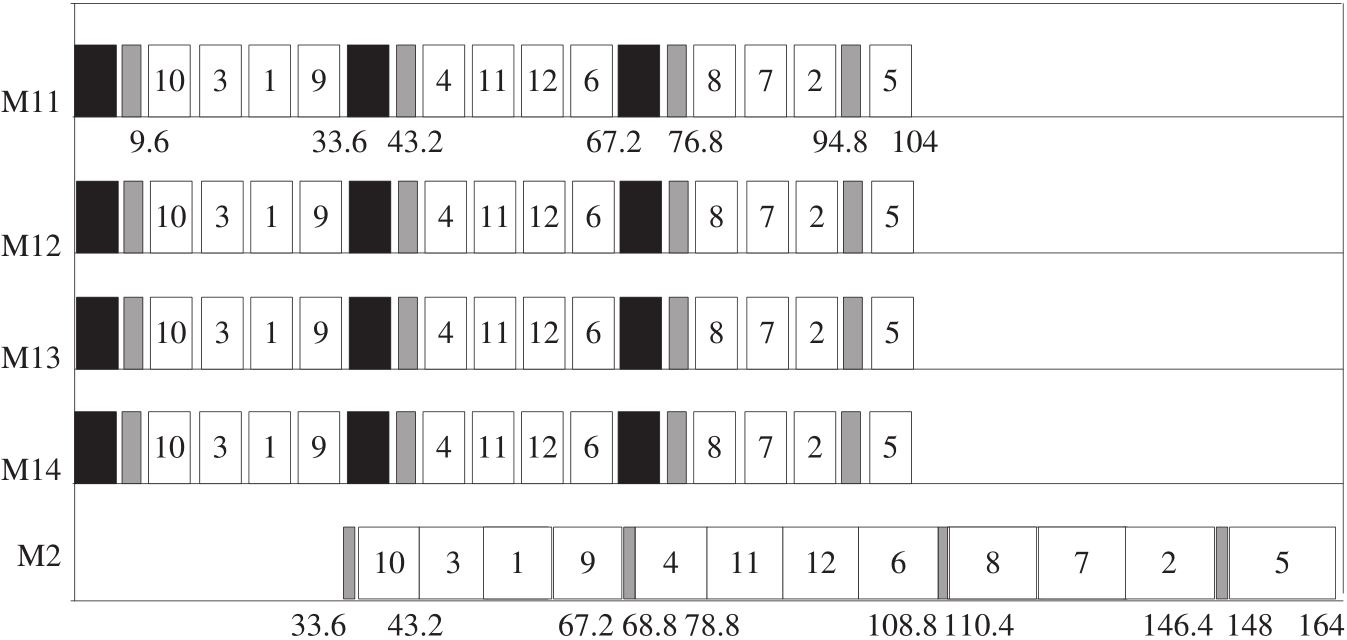
\includegraphics[width=10cm]{ganttexam1.jpg}
\caption{例\ref{exam:1}最优调度的Gantt 图\label{fig:gantt1}}
\end{figure}

这个MIP 公式可以用来求解只有少量的作业和产品簇,对于通常问题的调度求解十分困难。实际情况中,我们可能遇到大量作业和产品簇的问题,所以建立启发式方法变得十分重要,这些方法可以较快解决中、大型问题的近似最优解。

\ksection{启发式方法}
在2.5节中,我们解释了现行的单件处理和EDD 规则调度方法。为了有效解决涌现的问题和提高调度效果,我们提出了启发式方法。
\newcommand{\Step}{{\heiti 步骤}}

\ksubsection{启发式方法1:FBEDD}
我们将EDD 规则结合完整批的性质,建立了一个完整批EDD (FBEDD)启发式方法,以最小化目标值,具体步骤如下

\begin{asparaenum}
\renewcommand{\labelenumi}{\heiti 步骤\theenumi~}
\item 置$S=\phi,\ S_U = \{J_1,J_2,...,J_n\},\ B=\phi,\ i=1,2,...,b,\ b = n/c$。
\item 将$S_U$中的作业按$d_j$非减的顺序排列,置$i=1$。
\item 将$S_U$中的前$c$项作业组成批次$B_i$,即$B_i = \{J_{[1]},...,J_{[c]}\}$。
\item 如果$S_U = \phi$,则执行\Step5,否则$i=i+1$,并执行\Step 3。
\item 最终的调度为$S=B=(B_1,...,B_b)$。
\end{asparaenum}

\ksubsection{启发式方法2:FBFS}
作业要群组成一些产品簇的集合。我们选用同簇中的$c$项作业组成一个完整批,然后把不同簇中剩余的作业组成最后一批,这批的作业按最短处理时间(SPT)规则排序。这个启发式方法的步骤叫做完整批簇排序(FBFS)启发式算法,如下所示。其中$\# F^f$表示产品簇作业$f$的集合$F^f$的作业数量。
\begin{asparaenum}
\renewcommand{\labelenumi}{\heiti 步骤\theenumi~}
\item 置$S_1 = \phi,\ S_2=\phi,\ S_U = \{J_1,...,J_n\},\ B = \phi,\ B' = \phi,\ b=n/c$。
\item 将$S_U$中的作业按$d_j$非减的顺序排列。
\item 将得到的序列作业按产品簇排序以组成集合,置$f=1$。
\item 如果$\# F^f \geqslant c$,执行\Step 7,否则执行\Step 5。
\item 置$i=1$,将$F^f\text{并入}B'_i$作为一个局部批,然后从$S_U\text{剔除}B'_i$。
\item 如果$S_U = \phi$,执行\Step 9,否则置$f=f+1$,并执行\Step 4。
\item 置$i=1$,从$F^f$中拿出前$c$项作业作为一个完整批$B^f_i$,将至并入$B$,并从$S_U\text{中剔除}B^f_i$。
\item 如果$\# F^f \geqslant c$,执行\Step 7,否则执行\Step 5。
\item 置$B = \{B_1^1,...,B_i^1,...,B_1^4,...,B_i^4\},\ B' = \{B'_1,...,B'_4\}$。按$p_{2j}$非减的顺序排列重排$B'$中的作业。
\item 在作业顺序不变的情况下,重新定$B\text{与}B'$中的指数。置$B=\{B_1,...,B_{k-1}\}\text{并且}B' = \{B_k,B_{k+1},...,B_b\}$均为完整批。
\item 最终调度为$S=B\cup B' = \{B_1,B_2,..,B_b\} = \{J_{[1]},J_{[2]},...,J_{[n]}\}$。
\end{asparaenum}

我们来解释以上的步骤。在\Step1和\Step2中,我们构建了一个初始调度,作业是按EDD 规则排序的。在\Step3中,作业群组成4个簇。\Step4 -- 8,我们取各簇前$c$项作业组成一个完整批,并将剩余的作业组成一个最后批。在\Step9,我们按SPT 规则重排了局部批的作业,以改良目标函数值。\Step10我们在不改变作业顺序的情况下,重新设置了各完整批的指数,以保证其完整。在\Step11,我们得到了最终调度方案。
\begin{example}
考虑一个12个作业的问题,其中$p_{aj}=9,s_a=5.2,p_{1j}=24,s_b=6.4,s_{f1}=3.2,s_{f2}=1.6$。其他数据同例\ref{exam:1}。
\end{example}
\begin{asparaenum}
\renewcommand{\labelenumi}{解\theenumi:}
\item 用EDD 规则求解该问题,得到最终调度:$C_{\max}=211,\ \sum C_j = 1419.0,\ \sum T_j = 66.2,\ Z(S)=408.32$。
\item 用FBEDD 规则求解该问题,得到最终调度:$C_{\max}=178.4,\ \sum C_j = 1344.4,\ \sum T_j = 0,\ Z(S)=375.92$。
\item 用FBFS 规则求解该问题,得到最终调度:$C_{\max}=164,\ \sum C_j = 1163.2,\ \sum T_j = 0,\ Z(S)=331.04$。
\end{asparaenum}
\ksubsection{启发式方法3:RFBFS}
当我们运用FBFS 求解大型问题的时候,换线时间和可以被最小化,然而,这个方法给出了同簇产品的优先级,却不顾工期。因此,这可能会耗费许多时间处理同簇产品的批次,导致一些作业被提前完成,而一些作业却要滞后完成。为了改善FBFS 的这个不足,我们融入了滚动时域调度策略以达成滚动完整批产品簇调度(RFBFS)的启发式方法。RFBFS 将大型问题分割成多个EDD 序列的小型问题,然后重复执行FBFS 直到所有作业都被调度。
由于RFBFS 运行FBFS 处理小型短时域问题,这样可以用于处理大型问题。该启发式方法的步骤如下,其中$n_b$表示每月可处理的批数。
\begin{asparaenum}
\renewcommand{\labelenumi}{\heiti 步骤\theenumi~}
\item 置$S_1 = \phi,\ S_U = \{J_1,...,J_n\},\ B_1 = \phi,\ B'_1 = \phi,\  n = b \times c$。
\item 将$S_U$中的作业按$d_j$非减的顺序排列,并置$\nu = 1$。
\item 从$S_U$中拿出前$n_b/2$项作业来执行FBFS,并产生一个局部调度$S_1 = B_1 \cup B'_1$。然后,置$\nu = \nu + 1$,并把剩下的$n_b/2$项作业执行FBFS,产生下一个局部调度$S_2 = B_2 \cup B'_2$。
\item 如果$S_U=\phi$,执行\Step5,否则,置$\nu = \nu + 1$,执行\Step3。
\item 最终的调度为$S=S_1\cup S_2\cup...\cup S_{\nu}$。
\end{asparaenum}

\ksection{确定下界}
为了评估启发式方法得到结果的质量,本节将引出下界。由于这些都是多目标函数,所以下界包含3个部分:\begin{inparaenum}[(1)]
\item $C_{\max}\text{的下界}LB_1$;
\item $\sum C_j\text{的下界}LB_2$;
\item $\sum T_j\text{的下界}LB_3$。
\end{inparaenum}
\renewcommand{\labelenumi}{}
\begin{asparaenum}
\item $C_{\max}\text{的下界}(LB_1)$
\suspend{asparaenum}

Ahmadi(1992)提出了LPT-Johnson 法则以最小化处理多簇产品的离散批系统的制造期。根据这个法则,作业在工段2按处理时间排列为非增序列。
为了得到合理的下界,我们融入了Azizoglu 和Webster(2003)提出的获得下界进程。
我们考虑将批换线时间$s_b$和产品簇换线时间$s_{f1}$计入工段1的处理时间,放宽工段2产品簇换线时间。
这样一来,下界可以由制造期加最小工段2簇换线时间($f_n \times s_{f2}$)得到。
记$C_{2,[j]}$(LPT)为$H_{[j]}$在工段2的完工时间,$f_n$为所有作业簇的数量,即:
\begin{numcases}{}
C_{2,[1]}(LPT) = (s_b + s_{f1} + p_1) + p_{2,[1]}\notag\\
C_{2,[j]}(LPT) = C_{2,[j-1]} + p_{2,[j]},\quad j=2,...,n\notag\\
LB_1 = C_{2,[n]}(LPT) + f_ns_{f2}\notag
\end{numcases}
\resume{asparaenum}
\item $\sum C_j\text{的下界}(LB_2)$
\suspend{asparaenum}

Ahmadi(1992)同时也提出完整批最短处理时间(Full Batch-SPT)法则以最小化工段2无闲置的离散批系统完工时间和。
根据这个法则,作业在工段2按处理时间排列为非减序列。
记$C_{2,[j]}$(SPT)为作业在工段2的完工时间,这样一来下界可由完工时间和加上工段2最小簇换线时间得到。簇换线时间只有在首个作业和末尾作业$f_n-1$时才考虑,即:
\begin{numcases}{}
C_{2,[1]}(SPT) = s_b + s_{f1} + p_1 + p_{2,[1]}\notag\\
C_{2,[j]}(SPT) = C_{2,[j-1]} + p_{2,[j]},\quad j=2,...,(n-f_n+1)\notag\\
C_{2,[j]}(SPT) = C_{2,[j-1]} + s_{f2} + p_{2,[j]},\quad j=(n-f_n+2),...,n\notag\\
LB_2 = \sum_{j=1}^n C_{2,[j]}(SPT) + (n+\sum_{k=1}^{f_n}(f_n-k))s_{f2}\notag
\end{numcases}
\resume{asparaenum}
\item $\sum T_j\text{的下界}(LB_3)$
\end{asparaenum}

Baker 和Martin(1974)证明SPT序列最小化了当所有作业都滞后的单机器滞后时间和。在这个离散批系统中,批处理时间相同,这样考虑由此引起的滞后和时,这个系统可以考虑为单个机器。
记$C_{2,[j]}$(SPT)为完工时间,$d_{[j]}$为SPT 顺序下$J_{[j]}$的工期。
这样一来,滞后时间和的下界可以由放宽所有作业皆滞后的约束得到,即:
\begin{numcases}{}
T_j = \max \{C_{2,[j]}(SPT)-d_{[j]}(SPT),0\},\quad j=1,...,n \notag \\
LB_3 = \sum_{j=1}^n T_j\notag
\end{numcases}

将这3个独立的下界综合,可以得到该问题的下界:
\[ LB = \alpha LB_1 + \beta LB_2 + \gamma LB_3
\]

为了评估启发式算法求解的质量,我们用相对误差(RER)定义启发式方法和下界的差别:
\[
RER = \left( \frac{Heuristic_i - LB}{LB}\right)\times 100\%
\]
其中$Heuristic_i$是各启发式方法的目标函数值。
\begin{example}
举一个下界的例子,考虑一个12个作业的问题,其中$p_{1j}=24,s_b=6.4,s_{f1}=3.2,s_{f2}=1.6$,其他数据同例\ref{exam:1}。
\end{example}

在参数为$(\alpha,\beta,\gamma)=(n/2,2,2)$的情况下,得到的下界为:
\begin{align*}
LB &= 0.6 \times LB_1 + 0.2 \times LB_2 + 0.2 \times LB_3 \\
& =0.6 \times 164 + 0.2 \times 1152 + 0.2 \times 0\\
& = 328.8 
\end{align*}
3种启发式方法的相对误差如下:
\begin{align*}
RER_{EDD} & = \left(\frac{408.32-328.8}{328.8}\right)\times 100 \% = 24.18 \%\\
RER_{FBEDD} & = \left(\frac{375.92-328.8}{328.8}\right)\times 100 \% = 14.33 \%\\
RER_{FBFS} & = \left(\frac{311.04-328.8}{328.8}\right)\times 100 \% = 24.18 \%
\end{align*}

从结果来看,$RER_{FBFS}$的值较小,说明由FBFS 得到的结果质量明显要优于EDD 和FBEDD。

% !Mode:: "TeX:UTF-8"
% !TEX root = ..\Literature_Translation.tex
\kchapter{计算实验}
在本章,将通过计算实验来评估MIP 模型和所提出的启发式算法的运行情况。
参考实际数据\reft{tab:2yearproduction},装配车间每月大约能装配24件作业,故实验可以通过3部分进行:\begin{inparaenum}[(1)]
\item 时间域为$2$周的包含$n=12$件作业的小型问题;
\item 时间域为$1\text{或}2.5$月的包含对应$n=24\text{或}n=60$件作业的中型问题;
\item 时间域为$4,8,12$月的包含对应$n=100,200,300$件作业的中型问题。
\end{inparaenum}
所有启发式方法皆用MATLAB 语言编写程序,并在处理器为AMD Athlon 2.91 GHz 的PC 上运行。
\ksection{评估小型问题}
我们随机产生10个12件作业和4个产品簇的示例($N=10$),其中$f_j$由均匀分布$DU(1,4)$产生,$d_j$由均匀分布$DU(100,180)$产生。
为了评估这些启发式方法的效果,考虑两个度量方面:求解质量和运行时间(Hamta,2012)。
为了检测启发式方法的求解质量,我们可以计算平均百分相对偏差(ARPD)如下(Laha 和Sarin,2009):
\[ARPD = \frac{100}{N}\sum_{i=1}^N\left(\frac{Heuristic_i - Optimal_i}{Optimal_i}\right)
\]
其中,$Heuristic_i$是第$i$个示例用启发式方法得到的目标函数值,$Optimal_i$是其MIP 目标函数值。
我们计算3个启发式方法EDD,FBEDD 和FBFS 按$(\alpha,\beta,\gamma)=(n/2,2,2)=(12/2,2,2)=(0.6,0.2,0.2)$加权的目标函数值和ARPD 的结果如\reft{tab:comparisonforarpd}所示。
\begin{table}[h]
  \centering\xiaowu
  \caption{MIP 和3个启发式方法的ARPD 比较}
    \begin{tabular}{ccccccccc}
    \toprule
    \multirow{2}[4]{*}{示例编号} & \multicolumn{2}{c}{MIP} & \multicolumn{2}{c}{EDD} & \multicolumn{2}{c}{FBEDD} & \multicolumn{2}{c}{FBFS} \\
   \cline{2-9}
          & Z     & time(s) & Z     & ARPD  & Z     & ARPD  & Z     & ARPD \\
      \midrule
    1     & 331.04 & 10    & 423.64 & 27.97 & 375.92 & 13.56 & 331.04 & 0 \\
    2     & 374.56 & 15    & 435.88 & 16.37 & 396.88 & 5.96  & 376.48 & 0.51 \\
    3     & 338.72 & 21    & 425.64 & 25.66 & 380.08 & 12.21 & 344.48 & 1.7 \\
    4     & 332.4 & 123   & 399.48 & 20.18 & 354.32 & 6.59  & 338.16 & 1.73 \\
    5     & 377.28 & 35    & 435.84 & 15.52 & 395.2 & 4.75  & 377.28 & 0 \\
    6     & 342.64 & 47    & 441.2 & 28.76 & 393.68 & 14.9  & 342.64 & 0 \\
    7     & 316.64 & 24    & 414.64 & 30.95 & 349.64 & 10.42 & 316.64 & 0 \\
    8     & 345.36 & 22    & 443.28 & 28.35 & 391.48 & 13.35 & 345.36 & 0 \\
    9     & 359.04 & 35    & 451.04 & 25.62 & 399.44 & 11.25 & 359.04 & 0 \\
    10    & 386.72 & 8     & 442.56 & 14.44 & 432.8 & 11.92 & 389.04 & 0.6 \\[3pt]
    平均值   & 350.44 & 34    & 431.32 & 23.38 & 386.94 & 10.49 & 352.02 & 0.45 \\
    \bottomrule
    \end{tabular}
  \label{tab:comparisonforarpd}
\end{table}
由最后一行各ARPD 可以看出,EDD 为$23.38\%$,在区间$(14.44,30.95)\%$中,FBEDD 为$10.49\%$,在区间$(4.75,14.90)\%$中,而FBFS 仅为$0.45\%$,在区间$(0,1.73)\%$中,较其他两者小,因此,FBFS 的运行效果要明显优于其他两个。
至于运行时间,MIP 每次需要$34\ s$,在区间$(8,123)\ s$中,而FBEDD 和FBFS 皆只需小于$0.3\ s$。综上所述,FBFS 是针对小型问题的好方法。
\ksection{评估中、大型问题}
考虑紧急插单的情况,设计成由$80\%$的MTO(面向订单生产)作业和$20\%$的MTS(面向库存生产)作业组成的中、大型问题。我们将最短交付期$D_j$设置成至少15天($15\times 8 = 120\ h$),最长交付期设置成1年($365\times 8 = 3000\ h$),所以,交付期期间为$[120,3000]\ h$。
工期$d_j$的确定基于交付期和能力限制,正常工期($d_j = D_j$)设置成基于普通能力,紧张工期($d_j = D_j - 40$)和松弛工期($d_j = D_j$)设置成基于稀缺和宽裕能力。

由于这个问题是NP 困难,我们不能在可接受的时间内找到中、大型问题的最优解。
为了评估启发式方法的求解质量,我们用相对误差(RER)来比较启发式方法和下界的差。进一步说,我们定义相对改善率(RIR)来比较启发式方法和现行方法的运行差异(Mokhtari,2010)。
\[RIR(\%) = \frac{100}{N}\sum_{i=1}^N \left(\frac{Heuristic_i - Best_i}{Best_i}\right)
\]
其中,$Heuristic_i$是用启发式方法的第$i$个示例的求解值,$Best_i$是示例中的最优值。

对于中、大型问题,需要测试15类问题、5类作业($n = 24,60,100,200,300$)和3个水准的工期(紧张(T),正常(N),松弛(L))的组合。
每一个问题都包含10个示例,其中$f_j$由$DU(1,4)$产生,对于5类作业,$D_j$分别由$DU(120,360),DU(120,270),DU(120,1120),DU(120,2120),DU(120,3000)$产生。
我们用3种启发式方法计算$n=24,d_j=D_j$,及权重为$(\alpha,\beta,\gamma)=(n/2,2,2)=(24/2,2,2)=(0.75,0.125,0.125)$的问题的下界和目标值,汇总RER 和RIR 见\reft{tab:comparen=24}。
\begin{table}[h]
  \centering\xiaowu
  \caption{通过10个示例比较$n=24, d_j = D_j$问题的三种启发式方法}
    \begin{tabular}{cccccccccc}
    \toprule
    \multirow{2}[4]{*}{示例编号} & 下界(LB)    & \multicolumn{3}{c}{目标值(Z)} & \multicolumn{3}{c}{RER (\%)} & \multicolumn{2}{c}{RIR (\%)} \\
    \cline{2-10}
          &       & (1) EDD & (2) FBEDD & (3) RFBFS &$\frac{(1) - LB}{LB}$ & $\frac{(2) - LB}{LB}$ & $\frac{(3) - LB}{LB}$ &$\frac{(1) - (3)}{(3)}$ & $\frac{(2) - (3)}{(3)}$ \\
          \midrule 
    1     & 661.5 & 953.4 & 748.9 & 698.9 & 44.13 & 13.22 & 5.66  & 36.41 & 7.15 \\
    2     & 723.3 & 1047.6 & 824.2 & 744.4 & 44.84 & 13.95 & 2.92  & 40.73 & 10.72 \\
    3     & 723.2 & 998.2 & 825.3 & 765.8 & 38.02 & 14.11 & 5.88  & 30.35 & 7.77 \\
    4     & 722.7 & 956.5 & 811.6 & 743.5 & 32.36 & 12.31 & 2.88  & 28.66 & 9.17 \\
    5     & 762.2 & 1029.9 & 898.9 & 808.5 & 35.12 & 17.94 & 6.07  & 27.38 & 11.18 \\
    6     & 661.2 & 918.9 & 733.4 & 683.9 & 38.98 & 10.92 & 3.43  & 34.37 & 7.24 \\
    7     & 761.1 & 963.3 & 846.8 & 791.3 & 26.58 & 11.26 & 3.97  & 21.74 & 7.01 \\
    8     & 732.8 & 997.7 & 850.3 & 790.6 & 36.15 & 16.03 & 7.89  & 26.19 & 7.54 \\
    9     & 748.4 & 934   & 830.9 & 791.3 & 24.8  & 11.03 & 5.73  & 18.03 & 5.01 \\
    10    & 663.9 & 934.8 & 742   & 709.9 & 40.8  & 11.76 & 6.92  & 31.68 & 4.53 \\[3pt]
    平均值   & 716   & 973.4 & 811.2 & 752.8 & 35.95 & 13.3  & 5.14  & 29.31 & 7.76 \\
    \bottomrule
    \end{tabular}
  \label{tab:comparen=24}
\end{table}
由最后一行可以看出,EDD 和FBEDD 分别有平均RER $35.95\%\text{和}13.30\%$,而RFBFS 为$5.14\%$。同时可以看出,RFBFS 比EDD 和FBEDD 好,因为两者的平均RIR 分别为$29.31\%\text{和}7.76\%$。因此,RFBFS 就求解质量将提高效果上来说要优于其余两者。



\kchapter{总结和展望}
我们在本文考虑了一个机械装配车间的调度问题,提出了作业划分和批量处理等策略以提高车间效率。
同时,也采用80/20 混合MTO/MTS 法则来处理紧急插单。建立MIP 模型和3个启发式方法(FBEDD、FBFS 和RFBFS)以求解目标为最小化加权制造期和、完工时间和与滞后时间和的装配车间调度问题。
计算实验表明,求解小型问题时FBFS 要优于其他方法,而在求解中、大型问题时,RFBFS 的求解质量高。

我们证明了RFBFS 可以应用于广泛的两阶段装配车间,改进启发式方法应用于多阶段装配工厂将会成为有用的拓展。
此外,由于绝大多数工厂仍采用MRP 滚动时域工期来调度作业,因此,如何在装配工厂实现周期性调度便成为了未来研究的重要主题。


	% !Mode:: "TeX:UTF-8"
% !TEX root = ..\Literature_Translation.tex
\stepcounter{app}
\setcounter{figure}{0}
\setcounter{table}{0}
\newpage
\begin{Abstract}
\chapter*{航空工厂的装配夹具生产调度}\addcontentsline{toc}{section}{航空工厂的装配夹具生产调度}
\begin{center}
\vspace{2mm}
{
 {\xiaosi Bruno Jensen Virginio da Silva$^a$,  Reinaldo Morabito$^a$, Denise Sato Yamashita$^a$,\\ Horacio Hideki Yanasse$^b$}

 {\xiaowu $^a$Departamento de Engenharia de Produção, Universidade Federal de São Carlos, Brazil\\
 $^b$Nati Instituto de Ciência e Tecnologia, Universidade Federal de São Paulo, Brazil}
}
\end{center}
{\songti
\noindent \xiaowu\textbf{摘要:}我们将在本文研究在航空工厂的装配生产调度问题。飞机零件需要在夹具上生产制造,这在飞机制造上是很常见的,而且会由多个
工作站组成。由于夹具的物理工件小,当一个工作站在工作的时候,与其相邻的工作站便无法工作,这些约束称为邻接约束。该装配夹具调度问题的研究背景是,将员工的学习进程分为4个主要限制阶段(或时期)。最优化求解器和建模语言将运用到各阶段的数学建模和应用。该方法的计算实验将被运行在一个巴西航空工厂的案例研究,并可以得到该方法比现行方法要好的结论。

\keywords{生产调度、装配夹具、航空工厂、邻接约束}
}
\end{Abstract}

% !Mode:: "TeX:UTF-8"
% !TEX root = ..\Literature_Translation.tex
\kchapter{引言}
我们将在本文描述一个产生于飞机制造的装配夹具的生产调度问题。
我们对受邻接约束下,为了装配而用到夹具的这部分特殊飞机零件的生产特别感兴趣。夹具是用来夹紧工件或作为支撑的设备,专为适用特定零件或形状而建。
夹具的主要作用是定位,在某些情况下也用于整个加工操作中或其他工业过程的工件保持(Niu,1988;Drake,1989;Howe,2004)。
由于空间限制,夹具相邻的工作站不能同时开工,产生了邻接约束。
装配一个飞机零件至少需要2个步骤,其中之一需要在夹具上完成,另一个互补的装配操作将在工作台上进行。根据装配所需的零件,这两个操作需要重复操作。



% !Mode:: "TeX:UTF-8"
% !TEX root = ..\Literature_Translation.tex
\kchapter{阶段建模}
\ksection{阶段1}
阶段1的目标是找到只有1个装配夹具,而不顾可用工人数时的最大生产能力,即工人数量无限的情况下最小化制造期。
接下来的模型是基于Coffman(1976), Baker(1974), Morton和 Pentico(1993), Leung(2004)和 Pinedo(2008), Potts和 Strusevich(2009)的作业车间调度问题。设$L$为任务数,对于每个任务$j=1,2,...,J$:\\[3pt]
\indent$p_j:$ 任务$j$在装配夹具的操作持续时间\\
\indent$q_j:$ 任务$j$在工作台的操作持续时间

此外,需要对每个任务对$(j,k),j\neq k$定义集合如下:
\begin{numcases}{}
A = \left\{(j,k)\mid\text{任务$j$需在任务$k$开始前结束}\right\}\notag\\
B = \left\{(j,k)\mid\text{任务$j$和任务$k$在夹具内的邻接工作台操作}\right\}\notag\\
C = \left\{(j,k)\mid\text{任务$j$和任务$k$在夹具内同一个位置操作}\right\}\notag
\end{numcases}

决策变量建模如下:
\vspace{-3pt}
\begin{numcases}{y_{jk} = }
1\qquad\text{如果任务$j$在任务$k$前调度}\notag\\
0\qquad\text{其他情况}\notag 
\end{numcases}

$t_j:$ 任务$j$的开始时间

$t_F:$ 制造期

那么阶段1的数学模型如下:
\begin{align}
&\label{equb:1} \min \quad t_f \\
&\label{equb:2} t_j + p_j + q_j \leqslant t_F \qquad j = 1,...,J\\
&\label{equb:3} t_k + M(1 - y_{jk}) \geqslant t_j + p_j \qquad \text{对于所有} (j,k)\in C\\
&\label{equb:4} t_j + M\times y_{jk} \geqslant t_k + p_k \qquad \text{对于所有} (j,k)\in C\\
&\label{equb:5} t_k \geqslant t_j + p_j + q_j  \qquad \text{对于所有} (j,k)\in A\\
&\label{equb:6} t_k + M(1 - y_{jk}) \geqslant t_j + p_j \qquad \text{对于所有} (j,k)\in B\\
&\label{equb:7} t_j + M\times y_{jk} \geqslant t_k + p_k \qquad \text{对于所有} (j,k)\in B\\
&\label{equb:8} t_j \geqslant 0,\ y_{jk}\in \{0,1\},\quad j=1,...,J,\quad k=1,...,J,\quad j\neq k
\end{align}

在模型(\ref{equb:1}) -- (\ref{equb:8})中,目标函数\eqref{equb:1}最小化了制造期$t_F$,约束\eqref{equb:2}保证了制造期要不小于任何调度内任务的完成时间。
约束\eqref{equb:3}和(\ref{equb:4})避免了在同个装配工作站的任务重叠,需要注意的是,这两约束只为同工作站装配任务对$j$和$k$定义。
也需注意的是约束\eqref{equb:3}和(\ref{equb:4})是相互分离的,即一个激活时,另一个是冗余的,反之亦然(William,1999)。
参数M 是一个足够大的正数,可以定义为:$\sum_{j=1}^J(p_j + q_j)$。
约束\eqref{equb:5}保证先后之间的关系。
约束\eqref{equb:6}和(\ref{equb:7})保证需要用到邻接工作站的任务不会同时被调度。
约束\eqref{equb:8}参考决策变量的定义域。

以防万一,包括一些任务可能在0时刻之后提交,并且有些任务可能有工期(即防止任务与多于1架飞机有关而产生不同的工期),我们可以定义:\\[3pt]
\indent $r_j:$ 任务$j$的提交日期

$d_j:$ 任务$j$的工期\\
这样一来上述模型可以简单地改变以包含下述约束:
\begin{align}
&\label{equb:9} t_j \geqslant r_j \qquad \text{对于一些$j$}\\
&\label{equb:10} t_j + p_j + q_j \leqslant d_j \qquad \text{对于一些$j$}
\end{align}
其中,\eqref{equb:9}保证每一个任务$j$都在其提交日期$r_j$之后才被调度,\eqref{equb:10}保证每个任务$j$都在工期$d_j$前完成。
同时注意参数M 需要相应修改以使提交日期$r_j$非空。

\ksection{阶段2}
在本阶段,要考虑2个装配队伍:夹具装配队伍和工作台队伍。
该阶段的目标是最小化总成本或人工数量,并且在给定工期前完成。
在一些变化后,该问题可以建模成考虑时间因素的项目调度问题。
这个项目包含多个活动,每个活动都需要1种以上的资源使其得以执行。
通常,活动有其已知的持续时间,并且由于技术限制,它们中间往往存在先后关系。
本文研究的项目调度问题考虑有限但可再生资源,即被使用过后,该资源可以再次被使用(员工、机器设备等都是可再生资源的例子)。
其目标是在最小化资源使用量,考虑活动的先后关系,可用资源量,以及在给定工期的前提下,找到一个可行调度。
在项目调度的范畴中,该问题以时间约束的项目调度闻名(Brucker, Drexl, Mohring, Neumann,和Pesch, 1999; Yamashita和 Morabito, 2009)。
回顾项目调度问题可见Brucker等(1999), Hartmann和 Kolisch(2000), Kolisch和 Padman(2001), Guldemond, Hurink, Paulus,和 Schutten(2008)的文章。

将项目调度问题和本文研究的邻接约束调度问题相互对应并不困难,可将每个装配操作对应成活动,这样的话操作的时间(在夹具或工作台中)对应成活动的持续时间,操作所遵守的顺序(见\reff{fig:subsetoperation})对应活动的先后关系。
阶段1模型将2个操作对应1个任务,与之不同的是阶段2模型中1个操作对应1个活动。该模型需要10种类型的资源:
\begin{asparaenum}[(a)]
\item 夹具中的工人;
\item 工作台上的工人;
\item 8个夹具中各自的工作站。
\end{asparaenum}

在本阶段,在夹具和在工作台的工人数量可得。另一方面,对应于需要用到的工作站数量的资源类型是本问题的参数。
为了在该模型中正确描述邻接约束,可以人工假设每个对应到夹具工作站的资源类型用有2个可用单元,并且在这些夹具上处理的活动需要从工作站上获取2个资源,加上相邻两工作站间的1个资源。
\begin{figure}[h]
\centering\caption{装配夹具的工作站使用和资源的表示\label{fig:representationofresourcesandworkstations}}
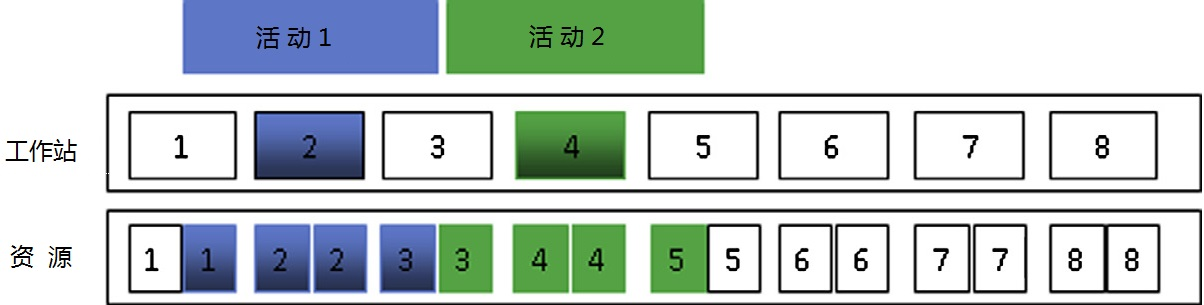
\includegraphics[width=12cm]{resourceandworkstation}
\end{figure}
\reff{fig:representationofresourcesandworkstations}举了一个例子,其中活动1在工作站2进行装配,它占用了2个工作站2的资源,其中1个是来自邻接工作站1,另一个来自邻接工作站3。
类似的,活动2占用2个工作站4的资源,其中1个来自邻接工作站3,另一个来自邻接工作站5。
因此,工作站1,3,5将被邻接约束所阻塞,不能和工作站2,4同时工作。
然而,任何使用工作站6,7,8的活动可以在处理活动1,2时同时进行。

进一步,整个调度周期可表示为多重时间周期$t = 1,...,T$,其中$T$表示每架飞机的生产周期。新增的参数模型如下:\\[3pt]
\indent $J:$ 活动数;

$T:$ 时间周期(时域)数;

$K:$ 夹具中的工作站数;

$W:$ 装配团队类型数;

$j:$ 活动,$j = 1,...,J$;

$t:$ 时间,$t = 1,...,T$;

$k:$ 资源类型,对应于各夹具的工作站,$k = 1,...,K$;

$w:$ 装配团队类型,$w = 1,...,W$;

$c_{jk}:$ 需要执行活动$j$的资源类型$k$的数量。注意$c_{jk} = 0$说明活动$j$没有在工作站$k$进行装配;

$C_k:$ 资源类型$k$的可用数量;

$p_j:$ 活动$j$的持续时间;

$n_{jw}:$ 需要执行活动$j$的类型$w$的工人数量;

$v_w:$ 装配队伍类型$w$的单位工人成本。

此外,对于每个活动对$(h,j)$,其中$h\neq j$,需要定义下面集合:
\begin{numcases}{}
H = \left\{(h,j)\mid\text{活动$h$先于活动$j$}\right\}\notag\\
G = \left\{(j)\mid\text{活动$j$在夹具上处理过,无论是哪个工作站}\right\}\notag
\end{numcases}

该模型的决策变量定义如下:
\begin{numcases}{x_{jt} = }
1 \qquad \text{如果活动$j$在时间$t$完成}\notag\\
0 \qquad \text{其他情况}\notag
\end{numcases}

$a_w:$ 类型$w$的资源需求量。特别的,由于模型用于求解阶段2,$W=2$,并且
\begin{center}
$a_1:$ 夹具内的工人需求量

$a_2:$ 工作台的工人需求量
\end{center}
如此一来,阶段2的数学模型如下:
\begin{align}
&\label{equb:11} \min \quad \sum_{w=1}^W v_wa_w\\
&\label{equb:12} \sum_{t=1}^T x_{jt} = 1,\qquad j = 1,...,J\\
&\label{equb:13} \sum_{t = r_h + p_h}^{d_h}t\cdot x_{ht}\leqslant \sum_{t = r_h + p_h}^{d_j}(t - p_j)x_{jt},\qquad \forall (h,j) \in H\\
&\label{equb:14} \sum_{j\in G}\sum_{b=t}^{\min\{t + p_j,T\}}c_{jk}x_{jb} \leqslant C_k,\qquad k = 1,...,K,\ t = 1,...,T\\
&\label{equb:15} \sum_{j=1}^J\sum_{b=t}^{\min\{t + p_j,T\}}n_{jw}x_{jb} \leqslant a_w,\qquad w = 1,...,W,\ t = 1,...,T\\
&\label{equb:16} x_{jt}\in \{0,1\},\ a_w\in Z^+,\ j = 1,...,J,\ t = 1,...,T,\ w = 1,...,W
\end{align}
在该模型中,目标函数(\ref{equb:11})最小化总人工成本,约束\eqref{equb:12}确保了每一个活动在水平时域中只调度过1次,约束\eqref{equb:13}确保各活动的先后关系,约束\eqref{equb:14}确保各资源的使用总和不超过其可利用值,\eqref{equb:15}确保各周期内的活动有充足的人工,\eqref{equb:16}参考决策变量的定义域。

注意每个周期$t$,约束\eqref{equb:14}和(\ref{equb:15})的左侧考虑了所有活动$j$在周期$t$前开始,并在$t$完成,即在区间$[t,t+p_j-1]$内完成,如\reff{fig:notinparallelt}所示。
\begin{figure}[h]
\centering\caption{在不平行的持续时间$t$内的活动\label{fig:notinparallelt}}
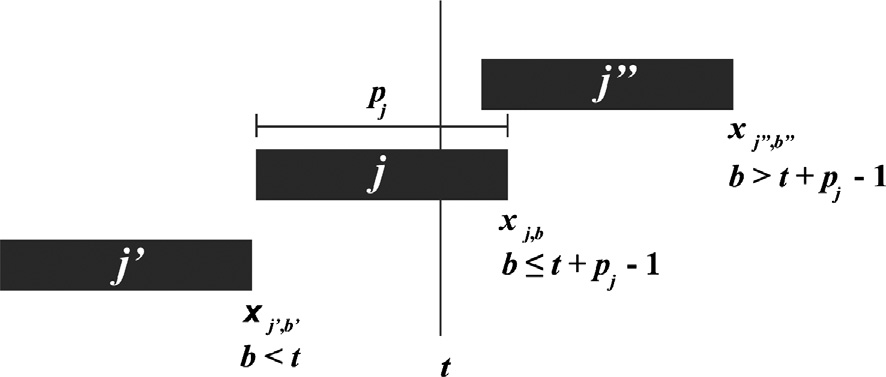
\includegraphics[width=8cm]{activitiesnotinparallel}
\end{figure}
如果在某个活动没有在周期$t$内处理,如$j'$和$j''$,那么它们不用在\eqref{equb:15}和(\ref{equb:15})的左边考虑。

需要考虑以下参数:\\[3pt]
\indent $EF_j:$ 活动$j$的最早可完成时间,表示在不考虑资源约束的先后关系;

$LF_j$活动$j$的最迟完成时间,不考虑项目延迟、先后关系和资源限制。

为防止某些活动的提交时间大于0,或者工期小于制造期(即防止与活动相关多架飞机,并且工期不同),我们需要定义:\\[3pt]
\indent $r_j:$ 活动$j$的可开始处理时间($r_j\geqslant EF_j - p_j$);

$d_j:$ 活动$j$的工期($d_j \leqslant LF_j$)。

所以上述模型可以简单地通过删除\eqref{equb:13}并增加下面的约束进行修改:
\begin{align}
&\label{equb:17}\sum_{t = \max\{EF_h,r_h + p_h\}}^{\min\{LF_h - 1,d_h - 1\}}t\cdot x_{ht}\leqslant \sum_{t =  \max\{EF_h,r_h + p_h\}}^{\min\{LF_h - 1,d_h - 1\}}(t - p_j)x_{jt} \qquad \forall (h,j)\in H\\
&\label{equb:18}x_{jt} = 0 \qquad t = 1,...,EF_j - 2,\ t = LF_j +1 ,...,T,\ j =1,..,J
\end{align}
其中,\eqref{equb:17}确保了所有活动的先后关系,约束\eqref{equb:18}确保了活动在其提交期和工期中被调度。这样可以在模型求解前消除已知值得变量,提高计算速度。

\eqref{equb:11} -- (\ref{equb:16})可以在离散时间内简单地改编成\eqref{equb:1} -- (\ref{equb:9})。由于在阶段1对劳动力没有限制,\eqref{equb:15}可以去除,目标函数(\ref{equb:11})可以写作:
\[ \centering\min\sum_{t=1}^T t\cdot x_{jt}
\]
其中$J$是先后关系网中的最后一个活动,然而,该模型并不完善,因为连续时间模型可以提供更短的计算运行时间。

\ksection{阶段3}
在阶段3,工人将分成两组,可在夹具内和工作台内操作的非专位组和只能在在工作台操作的专位组。此外,如阶段2模型所用到的参数,此处亦需考虑参数如下:\\[3pt]
\indent $s_{jw}:$ 需要在夹具内操作的活动$j$所需的$w$型资源数量;

$v_{jw}:$ 需要在工作台内操作的活动$j$所需的$w$型资源数量。

本文所研究的$j$操作问题只由单工人完成,因此$s_{jw}$和$v_{jw}$都等于1。阶段3的决策变量如下:
\begin{numcases}{x_{jt} = }
1 \qquad \text{如果活动$j$恰好在时间$t$完成}\notag\\
0 \qquad \text{其他情况}\notag
\end{numcases}\\[3pt]
\indent $a_w:$ 队伍$w$所需的工人数,在阶段3($W = 2$):

$a_1:$ 可以在工作台和夹具内操作的工人需求量;

$a_2:$ 只能在工作台操作而工人需求量。

需要注意的是,约束\eqref{equb:23}和(\ref{equb:24})引入了松弛变量$y_t$,表示在时间$t$可用于工作台的专位同人队伍冗余,阶段3的数学模型如下:
\begin{align}
&\label{equb:19} \min \qquad \sum_{w=1}^{W}v_wa_w\\
&\label{equb:20} \sum_{t = 1}^T x_{jt}  = 1,\quad j = 1,...,J\\
&\label{equb:21} \sum_{t = EF_h}^{LF_h -1}t\cdot x_{ht}\leqslant \sum_{t = EF_j}^{LF_j - 1}(t - p_j)x_{jt},\quad \forall (h,j) \in H\\
&\label{equb:22} \sum_{j\in G}\sum_{b=t}^{\min\{t + p_j-1,T\}}c_{jk}x_{jb}\leqslant C_k,\quad k = 1,...,K,\ t = 1,...,T\\
&\label{equb:23} \sum_{j\in G}\sum_{b=t}^{\min\{t + p_j-1,T\}}s_{jw}x_{jb} = a_w - y_t,\quad W = 1,\ t = 1,...,T\\
&\label{equb:24} \sum_{j\in J\backslash G}\sum_{b=t}^{\min\{t + p_j-1,T\}}v_{jw}x_{jb} = a_w + y_t,\quad W = 2,\ t = 1,...,T\\
&\label{equb:25} x_{jt} = 0,\qquad t = 1,...,EF_j - 2,\ t = LF_j +1 ,...,T,\ j =1,..,J\\
&\label{equb:26} x_{jt}\in \{0,1\},\ a_w \in Z^+,\ y_t \geqslant 0,\ t = 1,...,T,\ w = 1,...,W
\end{align}
目标函数(\ref{equb:19})最小化可用工人的总成本,\eqref{equb:20}保证了所有活动只被调度一次,\eqref{equb:21}保证了所有活动遵循其先后关系,\eqref{equb:23}确保了夹具内工人数量足够,\eqref{equb:24}确保了工作台内工人数量足够,\eqref{equb:25}修正了已知变量,\eqref{equb:26}参考变量的定义域。
注意在约束\eqref{equb:23}和(\ref{equb:24})中,$x_{jb},a_w,s_{jw},v_{jw}$为整数,保证了$y_t$的完整性。因此,\eqref{equb:26}中强调$y_t$是非负实数是必要的。

\ksection{阶段4}
在阶段4,装配组的所有工人可以在夹具和工作台内操作。由于工人间没有技能区别,为阶段2建立的数学模型可以用于这个阶段,在\eqref{equb:11} -- (\ref{equb:16})只要考虑一类工人($W = 1$)即可。这个阶段是学习曲线的最后阶段,所有工作都是多任务的。
在这个阶段,需要考虑较小增长的生产率,有着较大的影响。最优化队伍规模要比前阶段更为重要,因为这个阶段大部分飞机已完工。

% !Mode:: "TeX:UTF-8"
% !TEX root = ..\Literature_Translation.tex
\kchapter{计算结果}
使用建模语言GAMS(v23.0)建立该数学模型,并用CPLEX 11.2.1.0 使用4核求解。计算实验在一台处理器为Intel i7(2.8GHz, 12GB)的PC 机上运行,所有示例实验时间设为10 h。

这些示例包括15个活动,通常这些活动在工作台上的操作时间要长于夹具。
为了保护公司数据的隐私性,持续时间的单位(t.u.)不表示实际时间,因为其乘上了一个常数。需要注意的是,每架飞机需要两整套装配子集,因此,活动数目被扩大成30个活动。

\begin{table}[htbp]
  \centering
  \caption{Add caption}
    \begin{tabular}{ccccccc}
    \toprule

子集 &子集的零件 &活动(j) &\multicolumn{1}{m{20mm}}{夹具中的工作站} &\multicolumn{1}{m{20mm}}{夹具中的持续时间(mj)} &  \multicolumn{1}{m{20mm}}{工作台上的持续时间(qj)} &  \multicolumn{1}{m{20mm}}{前继活动(A(j,k)) }\\
\midrule
    1     & 1     & 1     & 1     & 5     & 7     & - \\
    1     & 1     & 2     & 1     & 4     & 47    & 1 \\
    2     & 1     & 3     & 1     & 5     & 7     & - \\
    2     & 1     & 4     & 1     & 4     & 47    & 3 \\
    1     & 2     & 5     & 2     & 15    & 29    & - \\
    1     & 2     & 6     & 2     & 9     & 71    & 5 \\
    2     & 2     & 7     & 2     & 15    & 29    & - \\
    2     & 2     & 8     & 2     & 9     & 71    & 7 \\
    1     & 3     & 9     & 3     & 11    & 40    & - \\
    2     & 3     & 10    & 3     & 11    & 40    & - \\
    1     & 4     & 11    & 4     & 12    & 40    & - \\
    1     & 4     & 12    & 4     & 6     & 40    & 11 \\
    2     & 4     & 13    & 4     & 12    & 40    & - \\
    2     & 4     & 14    & 4     & 6     & 40    & 13 \\
    1     & 5     & 15    & 5     & 8     & 30    & - \\
    1     & 5     & 16    & 5     & 6     & 40    & 15 \\
    2     & 5     & 17    & 5     & 8     & 30    & - \\
    2     & 5     & 18    & 5     & 6     & 40    & 17 \\
    1     & 6     & 19    & 6     & 12    & 17    & - \\
    1     & 6     & 20    & 6     & 6     & 40    & 19 \\
    2     & 6     & 21    & 6     & 12    & 17    & - \\
    2     & 6     & 22    & 6     & 6     & 40    & 21 \\
    1     & 7     & 23    & 7     & 7     & 12    & - \\
    1     & 7     & 24    & 7     & 7     & 30    & 23 \\
    2     & 7     & 25    & 7     & 7     & 12    & - \\
    2     & 7     & 26    & 7     & 7     & 30    & 25 \\
    1     & 8     & 27    & 8     & 10    & 61    & - \\
    1     & 8     & 28    & 8     & 12    & 66    & 27 \\
    2     & 8     & 29    & 8     & 10    & 61    & - \\
    2     & 8     & 30    & 8     & 12    & 66    & 29 \\
    \bottomrule
    \end{tabular}%
  \label{tab:addlabel}%
\end{table}%

\end{transcript}
\clearpage
